\documentclass{article}
\usepackage[dvips,a2paper,landscape,centering,margin=2cm]{geometry}
\usepackage{multicol}
\usepackage[utf8]{vietnam}
\usepackage{color}
\usepackage{amsmath, amsthm, amsfonts}
\usepackage{graphicx} 
\usepackage{enumitem}
\usepackage{enumerate}

\definecolor{azulillo}{rgb}{0.8,0.85,1}
\definecolor{marronrp3}{rgb}{.9,.9,.7}
\definecolor{salmon}{rgb}{1,.9,.8}
\definecolor{rojo}{rgb}{.6,.1,0}

\pagestyle{empty}

\def\to{\rightarrow}

% Hyphenation
\hyphenation{coa-gu-la-tion frag-men-ta-tion}

% ===========================================================================

\title{}
\author{}
\date{}

\begin{document}
%\maketitle
\Large
\begin{center}
  \begin{minipage}{.19\linewidth}
    \includegraphics[width=.5\linewidth]{logo.eps}
  \end{minipage}
  %&
  \begin{minipage}{.6\linewidth}
    \begin{center}
      \Huge \textbf{Evaluation of Polynomials by Computer}
    \end{center}
  \end{minipage}
  %&
  \hspace{.03\linewidth}
  \begin{minipage}{0.16\linewidth}
    \begin{flushright}
      Trương Nguyễn Thùy Trang - 21110691\\
      Đặng Công Tuấn - 21110709\\
      Lại Trọng Minh Trường - 21110934\\
      \vspace{.1cm} \small \emph{Đại học Sư Phạm Kỹ Thuật TP.HCM}\\
      \vspace{.1cm} \small \emph{Đề án cuối kỳ cấu trúc dữ liệu và giải thuật}\\
      \vspace{.1cm} \small \emph{Năm học 2022 - 2023}
    \end{flushright}
  \end{minipage}
\end{center}

\vspace{.1cm}

% ---------------------------------------------------------------------------

\setlength{\columnsep}{1cm}
\begin{multicols}{3}

\noindent
\fcolorbox{black}{salmon}{
  \begin{minipage}[t]{.96\linewidth}
    \vspace{.05cm}
    \begin{center}
      \vspace{.1cm}
      \section*{\Huge Kết quả chính}
      \Large Bài viết mô tả các phương pháp tối ưu để chuyển đổi bằng một cách nào đó thành số lượng
       phép nhân tối thiểu trong việc đánh giá đa thức bằng máy tính. Bài viết chỉ xem xét trường hợp
        đặc biệt nhất P = $y^n$ với ba thuật toán được đưa ra lần lượt là binary method, factor method, 
        tree method để tối ưu phép tính. 
    \end{center}
  \end{minipage}
}

\section*{\LARGE Binary method}

\qquad Một phương pháp khá nổi tiếng, (xem ví dụ, Floyd [ 1, trang 50—51 ]), 
  và có thể gọi là Binary Method, có thể được mô tả như sau:

    \begin{itemize}
    \item[a)] Viết n dưới dạng số trong hệ thống nhị phân, ví dụ: nếu n là 13 trong số thập phân, thì n là 1101 trong nhị phân.
    \item[b)] Thay thế mỗi "1" bằng SX và mỗi “0” bằng S; ví dụ: 1101 trở thành SXSXSSX.
    \item[c)] Hủy SX ở đầu bên trái. Chuỗi kết quả có thể được hiểu: S = "bình phương" và X = "nhân với y". Trong ví dụ của chúng tôi, 
    chúng tôi tính toán $y^{13}$ với chuỗi SXSSX:
    % \setmainfont{Consolas}
    \begin{itemize} % ra cái 1., 2.,...
        \item[1.] Lấy y;
        \item[2.] Bình phương (cho $y^{2}$ );
        \item[3.] Nhân với y (cho $y^{3}$ );
        \item[4.] Bình phương (cho $y^{6}$ );
        \item[5.] Bình phương (cho $y^{12}$ );
        \item[6.] Nhân với y (cho $y^{13}$ ).
      \end{itemize}
      % \setmainfont{<tên-phông>} 
  \end{itemize}
  \qquad Chúng tôi đã sử dụng 5 phép nhân, trong trường hợp này có thể được hiển thị là tối thiểu.

\section*{\LARGE Factor method}


\qquad Một thuật toán khác, được cho là mới, có thể được gọi là Factor Method. 
Ở đây chúng ta tạo ra các chuỗi S(n, m) như sau:
  \begin{itemize}
    \item[a)]	Nếu n không phải là số nguyên tố, S(n, m) = S(n/p,m)S(p, nm/p), trong đó p là thừa số nguyên tố nhỏ nhất của n.
    \item[b)]	Nếu n là số nguyên tố, S(n, m) = S(n - 1, m)$X_m$.
    \item[c)]	S(l, m) = chuỗi null.
  \end{itemize}
  \qquad Giải thích: $X_m$ có nghĩa là "nhân với $y^m$" , đó là một kết quả đã được 
  tính toán trước đó.  S(n, m) là chuỗi cho phép tính của $y^{mn}$ giả sử 
  rằng $y^m$ đã được tính toán. Mục tiêu là tìm S (n, 1).\\
  \indent \qquad Ví dụ:
  \begin{center}
    \begin{eqnarray}
      S(13, 1)  & = &S(12, 1)X_1 \\ 
        & = & S(6,1)S(2, 6)X_1 \\  
        & = & S(3,1)S(2, 3)X_6X_1 \\ 
        & = & S(2,1)X_1X_3X_6X_1 \\
        & = & X_1X_1X_3X_6X_1 
    \end{eqnarray}
  \end{center}
  \qquad Một cách khác để mô tả thuật toán này là:
  \begin{itemize}
    \item[a)] Phân tích n thành các số nguyên tố, n = $p_1p_2...p_r.$
    \item[b)] Nếu n là số nguyên tố, hãy tính $(y^{n-1})y$
    \item[c)] Nếu n là hợp số, hãy tính $(...((y^{p1})^{p2})...)^{pr}$
  \end{itemize}
\noindent

% ---------------------------------------------------------------------------

\section*{\LARGE Tree method}


  \qquad Tree Method - phương pháp phát triển một cái cây, là một trong những kỹ thuật tốt nhất 
  trong các kỹ thuật xử lý danh sách. Bắt đầu ở cấp độ 0 với một nút duy nhất có nhãn 1. Để đến 
  cấp độ tiếp theo khi một cấp độ được hoàn thành, hãy xử lý các nút ở cấp độ trước đó từ trái sang 
  phải. Đối với mỗi nút, hãy thử thêm từng giá trị phía trên nút này, liên tiếp từ trên cùng. Nếu thu
   được bất kỳ giá trị mới nào, chúng sẽ trở thành các nút phân nhánh sang cấp độ tiếp theo. Các 
   giá trị trùng lặp thu được sẽ bị loại bỏ.\\
  \indent \qquad Ví dụ: chúng ta có thể phát triển ba cấp độ như trong Hình 1. 
  Loại bỏ các giá trị là trùng lặp, chúng ta nhận được Hình 2. Thực hiện các bổ sung 
  thử nghiệm từ trên xuống dưới dẫn đến một cây tốt hơn nhiều so với việc tạo ra chúng 
  từ dưới lên trên. Tuy nhiên, phương pháp từ dưới lên trên thuận tiện hơn nhiều để lập 
  trình và nó có thể được sử dụng nếu các nhánh mới từ nút được gắn từ phải sang trái. Cây 
  bắt đầu trông như trong Hình 3.\\
  \begin{center}
    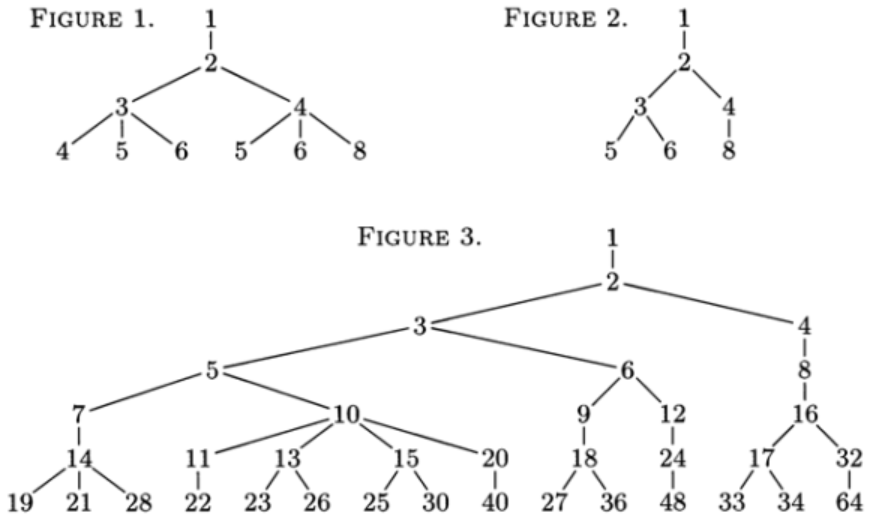
\includegraphics[width=.7\linewidth]{tree.png}\newline
  \end{center}

\noindent


\section*{\LARGE So Sánh giữa các phương pháp}
  \qquad Để so sánh hai phương pháp đầu, Binary Method sử dụng r + s - 1 phép nhân, trong đó r là số nguyên lớn nhất nhỏ hơn hoặc 
  bằng $log_2n$ và s là số thứ nhất trong biểu diễn nhị phân của n. Factor Method sử dụng phép nhân $M_n$, trong đó:
  \begin{center}
    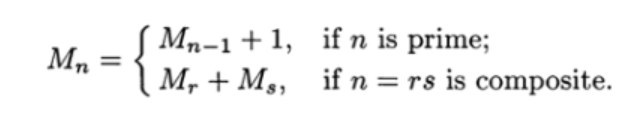
\includegraphics[width=.6\linewidth]{compair.png}
  \end{center}
  \qquad Factor Method tốt hơn một chút so với Binary Method nói chung:\\
  Đối với n $\leq$ 150, có:
  \begin{center}
    \begin{itemize}
      \item 93 trường hợp hai phương pháp bằng nhau,
      \item 32 trường hợp Factor method là tốt hơn 1 phép toán,
      \item 16 trường hợp Binary method là tốt hơn 1 phép toán,
      \item 8 trường hợp Factor method là tốt hơn 2 phép toán,
      \item 1 trường hợp (n = 129) Binary method là tốt hơn 2 phép toán.
    \end{itemize}
  \end{center}
  \indent \qquad Các trường hợp nhỏ nhất mà Factor Method vượt trội là n = 15, 27, 30, 31* , 39, 45. Các trường hợp nhỏ nhất mà Binary 
  Method vượt trội là n = 33, 49, 65, 66, 67, 69.\\
  \indent \qquad Nhưng có những trường hợp chúng ta có thể làm tốt hơn cả hai phương pháp. Đối với n $\leq$ 70, có 5 trường hợp được biết 
  đến mà điều này là đúng. (Chúng là n = 23, 43, 46, 47, 59).\\
  \indent \qquad Phương pháp thứ ba, là kỹ thuật tốt nhất mà tác giả biết đến, là Tree Method.
\noindent



\colorbox{marronrp3}{
  \begin{minipage}[t]{.96\linewidth}
    \vspace{.2cm}
    \centerline{\huge \textbf{Hướng phát triển}}
    \vspace{.05cm}

    \Large

    \qquad Chúng tôi chỉ tập trung vào tổng số phép nhân là tiêu chí của sự xuất sắc trong cuộc thảo luận này.\\
    \indent \qquad Binary method: Nếu n là một biến chưa biết, Binary method là ưu việt hơn. Trong thực tế, phương pháp đó
     rất phù hợp để kết hợp trong phần cứng của một máy tính nhị phân, như một toán tử lũy thừa.\\
    \indent \qquad Factor method: có giá trị khi n lớn và một sự ứng dụng đòi hỏi phải tính toán thường xuyên $y^n$.\\
    \indent \qquad Tree method: Nếu y là một số thực dấu phẩy động, tất nhiên có một điểm của quy luật hiệu suất giảm dần 
    (point of diminishing returns) khi n dần lớn, vì cuối cùng chúng ta sẽ tốt hơn bằng cách lấy logarit và 
    lũy thừa. Vì Tree method sử dụng r phép nhân ở cấp độ r, có thể ngừng tạo cây ở một mức nhất định; sau đó
     chúng ta có tập hợp tất cả các giá trị "thú vị" của n. Ví dụ, cây trong Hình 3 trong bài báo cho thấy tất
      cả n mà người ta biết rằng $y^n$ cần ít nhất là 6 phép nhân.

    \hspace{.05cm}
  \end{minipage}
}

\vspace{.5cm}

% ---------------------------------------------------------------------------
%
\small
\begin{thebibliography}{}


\bibitem Robert W. Floyd, \emph{"An algorithm for coding efficient arithmetic operations,"} Communications of the ACM 4 (1961), 42—51.
\bibitem A. M. Ostrowski, \emph{"On two problems in abstract algebra connected with Horner's rule,"} Studies in Mathematics and Mechanics 
Presented to Richard von Mises (New York: Academic Press, 1954),
\bibitem John Todd, A Survey of Numerical Analysis (New York: McGraw— Hill, 1962), 3-4.

\end{thebibliography}

\end{multicols}

\end{document}